\section*{Lecture 02: Galilean Stuffs}
\addcontentsline{toc}{section}{Lecture 02: Galilean Stuffs}
In the previous lecture, we saw how Newton's laws define an inertial frame and how we can rephrase the second and third law in terms of intertial frames, to avoid confusion. It happens that, there are reference frames where the first law doesn't hold true. \\[0.2cm]
Imagine a person inside a darkened car, isolated from the outside world, with a ball hanging from the roof of the car. The car suddenly starts accelerating and (as intuition speaks) the ball starts moving. The person claims "The ball has moved!" \emoji{skull}.\\[0.2cm] Note that from the perspective of the person, no force has been applied to the ball, yet it moved, which is a direct violation of the second law. Thus, we can call this frame \textit{non-inertial}. \\[0.2cm]
Now, consider a person inside an ill-fated lift, tragically falling \emoji{smiling-face-with-tear}.  Everything in the lift frame is accelerating together under gravity and hence `weightlessness' (free-fall) occurs. If somehow a coin is also there in the lift, it simply floats. And if the person pushes the coin, it moves with an almost constant velocity. Thus, it is a very good approximation to an \textit{intertial frame} (although, extremely tragic for the person!).
\begin{figure}[H]
    \centering 
    

\tikzset{every picture/.style={line width=0.75pt}} %set default line width to 0.75pt        

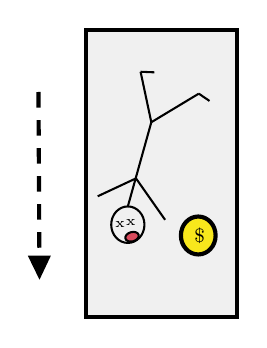
\begin{tikzpicture}[x=0.75pt,y=0.75pt,yscale=-1,xscale=1]
%uncomment if require: \path (0,201); %set diagram left start at 0, and has height of 201

%Shape: Rectangle [id:dp43885108717089105] 
\draw  [fill={rgb, 255:red, 155; green, 155; blue, 155 }  ,fill opacity=0.15 ][line width=1.5]  (219.87,46) -- (292.68,46) -- (292.68,184.55) -- (219.87,184.55) -- cycle ;
%Shape: Ellipse [id:dp6930955052406024] 
\draw   (232.05,139.91) .. controls (232.05,135.05) and (235.64,131.12) .. (240.06,131.12) .. controls (244.48,131.12) and (248.06,135.05) .. (248.06,139.91) .. controls (248.06,144.77) and (244.48,148.71) .. (240.06,148.71) .. controls (235.64,148.71) and (232.05,144.77) .. (232.05,139.91) -- cycle ;
%Straight Lines [id:da20965970546638646] 
\draw    (240.06,131.12) -- (251.37,90.56) ;
%Straight Lines [id:da10801740144899596] 
\draw    (251.37,90.56) -- (274.24,76.78) ;
%Straight Lines [id:da8911861421123949] 
\draw    (251.37,90.56) -- (246.2,66.24) ;
%Straight Lines [id:da28213518227119183] 
\draw    (258.01,137.57) -- (243.99,117.6) ;
%Straight Lines [id:da6534545499097717] 
\draw    (225.54,126.23) -- (243.99,117.6) ;
%Straight Lines [id:da3675373664676822] 
\draw    (279.4,80.29) -- (274.24,76.78) ;
%Straight Lines [id:da997055291906832] 
\draw    (252.84,66.51) -- (246.2,66.24) ;
%Shape: Ellipse [id:dp13846564322056798] 
\draw  [fill={rgb, 255:red, 208; green, 2; blue, 27 }  ,fill opacity=0.69 ] (238.87,146.51) .. controls (238.63,145.3) and (239.86,143.96) .. (241.63,143.52) .. controls (243.41,143.09) and (245.04,143.72) .. (245.29,144.93) .. controls (245.54,146.14) and (244.3,147.48) .. (242.53,147.92) .. controls (240.76,148.35) and (239.12,147.72) .. (238.87,146.51) -- cycle ;
%Shape: Ellipse [id:dp003301931365316424] 
\draw  [fill={rgb, 255:red, 248; green, 231; blue, 28 }  ,fill opacity=1 ][line width=1.5]  (265.62,145.12) .. controls (265.62,140.07) and (269.36,135.98) .. (273.99,135.98) .. controls (278.61,135.98) and (282.35,140.07) .. (282.35,145.12) .. controls (282.35,150.17) and (278.61,154.26) .. (273.99,154.26) .. controls (269.36,154.26) and (265.62,150.17) .. (265.62,145.12) -- cycle ;
%Straight Lines [id:da08779430940978317] 
\draw [line width=1.5]  [dash pattern={on 5.63pt off 4.5pt}]  (197,75.99) -- (197.48,162.42) ;
\draw [shift={(197.5,166.42)}, rotate = 269.68] [fill={rgb, 255:red, 0; green, 0; blue, 0 }  ][line width=0.08]  [draw opacity=0] (11.61,-5.58) -- (0,0) -- (11.61,5.58) -- cycle    ;

% Text Node
\draw (232.45,136.94) node [anchor=north west][inner sep=0.75pt]  [font=\tiny] [align=left] {x};
% Text Node
\draw (237.61,136.13) node [anchor=north west][inner sep=0.75pt]  [font=\tiny] [align=left] {x};
% Text Node
\draw (270.46,140.03) node [anchor=north west][inner sep=0.75pt]  [font=\scriptsize]  {$\$$};


\end{tikzpicture}

    \caption{A sad guy floating with a coin in a falling lift }
\end{figure}
\noindent
We had always wanted the physical laws to stay the same. This is actually the statement of Galilean relativity:
\begin{center}
    \itshape
    ``Laws of physics (nature) must be the same in all intertial frames of reference'' 
\end{center}
By physical laws, we imply Newton's laws of mechanics and the law of gravitation. To have a more mathematical (and less philosophical) aspect to the above statement, we define the \textit{Galilean transformation}.
\subsection*{Galilean Transformation}
\addcontentsline{toc}{subsection}{Galilean Transformation}
Let an onject be at point $P$ and consider two reference frames $O$ and $O'$, which coincided at $t=0$ but have moved apart since, along the common x-axis. (Henceforth, reference frames will simply be termed \textit{observers} ).
\begin{figure}[H]
    \centering 
    

\tikzset{every picture/.style={line width=0.75pt}} %set default line width to 0.75pt        

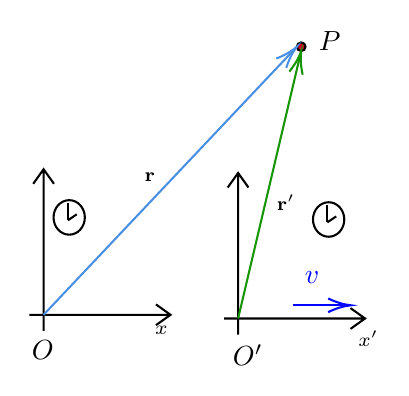
\begin{tikzpicture}[x=0.75pt,y=0.75pt,yscale=-1,xscale=1]
%uncomment if require: \path (0,273); %set diagram left start at 0, and has height of 273

%Shape: Axis 2D [id:dp6413064504443255] 
\draw  (172,234.23) -- (239.96,234.23)(178.8,164.12) -- (178.8,242.02) (232.96,229.23) -- (239.96,234.23) -- (232.96,239.23) (173.8,171.12) -- (178.8,164.12) -- (183.8,171.12)  ;
%Shape: Axis 2D [id:dp6848366837212227] 
\draw  (265.73,236.01) -- (333.68,236.01)(272.52,165.9) -- (272.52,243.8) (326.68,231.01) -- (333.68,236.01) -- (326.68,241.01) (267.52,172.9) -- (272.52,165.9) -- (277.52,172.9)  ;
%Straight Lines [id:da6301070438212596] 
\draw [color={rgb, 255:red, 0; green, 6; blue, 255 }  ,draw opacity=1 ]   (298.98,229.65) -- (324.84,229.65) ;
\draw [shift={(326.84,229.65)}, rotate = 180] [color={rgb, 255:red, 0; green, 6; blue, 255 }  ,draw opacity=1 ][line width=0.75]    (10.93,-3.29) .. controls (6.95,-1.4) and (3.31,-0.3) .. (0,0) .. controls (3.31,0.3) and (6.95,1.4) .. (10.93,3.29)   ;
%Shape: Circle [id:dp9011756976883052] 
\draw  [fill={rgb, 255:red, 208; green, 2; blue, 27 }  ,fill opacity=1 ] (300.83,105.08) .. controls (300.83,103.93) and (301.77,103) .. (302.92,103) .. controls (304.07,103) and (305,103.93) .. (305,105.08) .. controls (305,106.23) and (304.07,107.17) .. (302.92,107.17) .. controls (301.77,107.17) and (300.83,106.23) .. (300.83,105.08) -- cycle ;
%Straight Lines [id:da4904503688134786] 
\draw [color={rgb, 255:red, 74; green, 144; blue, 226 }  ,draw opacity=1 ]   (178.8,234.23) -- (299.46,106.54) ;
\draw [shift={(300.83,105.08)}, rotate = 133.38] [color={rgb, 255:red, 74; green, 144; blue, 226 }  ,draw opacity=1 ][line width=0.75]    (10.93,-3.29) .. controls (6.95,-1.4) and (3.31,-0.3) .. (0,0) .. controls (3.31,0.3) and (6.95,1.4) .. (10.93,3.29)   ;
%Straight Lines [id:da5226446595512337] 
\draw [color={rgb, 255:red, 22; green, 150; blue, 5 }  ,draw opacity=1 ]   (272.52,236.01) -- (302.46,109.11) ;
\draw [shift={(302.92,107.17)}, rotate = 103.27] [color={rgb, 255:red, 22; green, 150; blue, 5 }  ,draw opacity=1 ][line width=0.75]    (10.93,-3.29) .. controls (6.95,-1.4) and (3.31,-0.3) .. (0,0) .. controls (3.31,0.3) and (6.95,1.4) .. (10.93,3.29)   ;
%Shape: Ellipse [id:dp5368108252831854] 
\draw   (308.6,188.32) .. controls (308.6,183.72) and (311.98,180) .. (316.14,180) .. controls (320.31,180) and (323.68,183.72) .. (323.68,188.32) .. controls (323.68,192.91) and (320.31,196.63) .. (316.14,196.63) .. controls (311.98,196.63) and (308.6,192.91) .. (308.6,188.32) -- cycle ;
%Straight Lines [id:da9231878639896117] 
\draw    (315.52,189.68) -- (319.78,186.83) ;
%Straight Lines [id:da9902333944174619] 
\draw    (315.52,189.68) -- (315.52,181.36) ;
%Shape: Ellipse [id:dp24687330317421963] 
\draw   (183.6,187.32) .. controls (183.6,182.72) and (186.98,179) .. (191.14,179) .. controls (195.31,179) and (198.68,182.72) .. (198.68,187.32) .. controls (198.68,191.91) and (195.31,195.63) .. (191.14,195.63) .. controls (186.98,195.63) and (183.6,191.91) .. (183.6,187.32) -- cycle ;
%Straight Lines [id:da7625719815546823] 
\draw    (190.52,188.68) -- (194.78,185.83) ;
%Straight Lines [id:da11762110512093371] 
\draw    (190.52,188.68) -- (190.52,180.36) ;

% Text Node
\draw (303.23,212.08) node [anchor=north west][inner sep=0.75pt]  [color={rgb, 255:red, 0; green, 6; blue, 255 }  ,opacity=1 ]  {$v$};
% Text Node
\draw (171.64,245.22) node [anchor=north west][inner sep=0.75pt]    {$O$};
% Text Node
\draw (268.56,247.22) node [anchor=north west][inner sep=0.75pt]    {$O'$};
% Text Node
\draw (310,96.4) node [anchor=north west][inner sep=0.75pt]    {$P$};
% Text Node
\draw (231,238.4) node [anchor=north west][inner sep=0.75pt]  [font=\scriptsize]  {$x$};
% Text Node
\draw (329,240.4) node [anchor=north west][inner sep=0.75pt]  [font=\scriptsize]  {$x'$};
% Text Node
\draw (226,164.4) node [anchor=north west][inner sep=0.75pt]  [font=\scriptsize]  {$\mathbf{r}$};
% Text Node
\draw (289.72,174.99) node [anchor=north west][inner sep=0.75pt]  [font=\scriptsize]  {$\mathbf{r} '$};


\end{tikzpicture}

    \caption{Observing same point from two different frames}
    \label{fig:gal_rel}
\end{figure}
\noindent
Now, the distance between the origins of two frames, at time $t$, will be $R = vt$. Then accordingly, we can write the relation between the coordinates of the two observers as follows:
   \begin{center}
     \begin{minipage}{0.5\textwidth}
    \begin{align*}
        x' &= x-vt\\
        y'&=y\\
        z' &=z \\
        t'&=t
    \end{align*}
\end{minipage}\hfill
\begin{minipage}{0.5\textwidth}
    
    
    $\begin{pmatrix}
        t'\\x'\\y'\\z'
    \end{pmatrix} = \begin{pmatrix}
        1&0&0&0 \\
        -v&1&0&0 \\
        0&0&1&0 \\
        0&0&0&1 \\
    \end{pmatrix}    \begin{pmatrix}
        t\\x\\y\\z
    \end{pmatrix}$
\end{minipage}
   \end{center}
\textcolor{red}{\textbf{An important assumption:}} The Galilean transformation assumes a \textit{universal time}, that is, time elapsed on clocks in both frames are the same \footnote{This was perhaps a fair assumption since time, atleast in the philosophical aspect, has always seemed to be \textit{superior}. }.\\[0.2cm]
Now, it is not necessary for the observers to move along the $x$ axis only. Hence, generalising the transformation to arbitrary direction, we obtain:
$$t'=t\qquad \vb{r'} = \vb{r} - \vb{v}t$$
Now, let us look how the physical laws react under the Galilean transformation. 
\begin{itemize}
    \item \textbf{Law of Gravitation:}\\[0.2cm] 
    Consider the situation in the diagram below:
    \begin{figure}[H]
        \centering 
        

\tikzset{every picture/.style={line width=0.75pt}} %set default line width to 0.75pt        

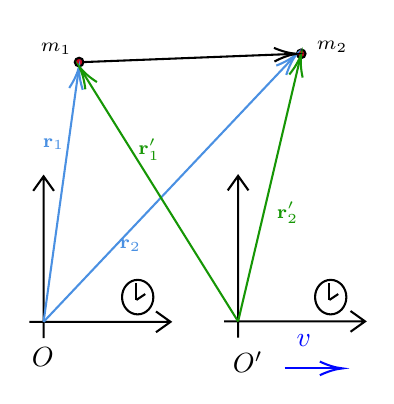
\begin{tikzpicture}[x=0.75pt,y=0.75pt,yscale=-1,xscale=1]
%uncomment if require: \path (0,186); %set diagram left start at 0, and has height of 186

%Shape: Axis 2D [id:dp22236225290792944] 
\draw  (225,146.23) -- (292.96,146.23)(231.8,76.12) -- (231.8,154.02) (285.96,141.23) -- (292.96,146.23) -- (285.96,151.23) (226.8,83.12) -- (231.8,76.12) -- (236.8,83.12)  ;
%Shape: Axis 2D [id:dp027564847074658116] 
\draw  (318.73,146.01) -- (386.68,146.01)(325.52,75.9) -- (325.52,153.8) (379.68,141.01) -- (386.68,146.01) -- (379.68,151.01) (320.52,82.9) -- (325.52,75.9) -- (330.52,82.9)  ;
%Straight Lines [id:da8338287582907346] 
\draw [color={rgb, 255:red, 0; green, 6; blue, 255 }  ,draw opacity=1 ]   (347.98,168.65) -- (373.84,168.65) ;
\draw [shift={(375.84,168.65)}, rotate = 180] [color={rgb, 255:red, 0; green, 6; blue, 255 }  ,draw opacity=1 ][line width=0.75]    (10.93,-3.29) .. controls (6.95,-1.4) and (3.31,-0.3) .. (0,0) .. controls (3.31,0.3) and (6.95,1.4) .. (10.93,3.29)   ;
%Shape: Circle [id:dp5997377273143482] 
\draw  [fill={rgb, 255:red, 208; green, 2; blue, 27 }  ,fill opacity=1 ] (353.83,17.08) .. controls (353.83,15.93) and (354.77,15) .. (355.92,15) .. controls (357.07,15) and (358,15.93) .. (358,17.08) .. controls (358,18.23) and (357.07,19.17) .. (355.92,19.17) .. controls (354.77,19.17) and (353.83,18.23) .. (353.83,17.08) -- cycle ;
%Straight Lines [id:da42368451729998724] 
\draw [color={rgb, 255:red, 74; green, 144; blue, 226 }  ,draw opacity=1 ]   (231.8,146.23) -- (352.46,18.54) ;
\draw [shift={(353.83,17.08)}, rotate = 133.38] [color={rgb, 255:red, 74; green, 144; blue, 226 }  ,draw opacity=1 ][line width=0.75]    (10.93,-3.29) .. controls (6.95,-1.4) and (3.31,-0.3) .. (0,0) .. controls (3.31,0.3) and (6.95,1.4) .. (10.93,3.29)   ;
%Straight Lines [id:da4528896382478149] 
\draw [color={rgb, 255:red, 22; green, 150; blue, 5 }  ,draw opacity=1 ]   (325.52,146.01) -- (355.46,19.11) ;
\draw [shift={(355.92,17.17)}, rotate = 103.27] [color={rgb, 255:red, 22; green, 150; blue, 5 }  ,draw opacity=1 ][line width=0.75]    (10.93,-3.29) .. controls (6.95,-1.4) and (3.31,-0.3) .. (0,0) .. controls (3.31,0.3) and (6.95,1.4) .. (10.93,3.29)   ;
%Shape: Ellipse [id:dp7373920249939159] 
\draw   (362.6,134.32) .. controls (362.6,129.72) and (365.98,126) .. (370.14,126) .. controls (374.31,126) and (377.68,129.72) .. (377.68,134.32) .. controls (377.68,138.91) and (374.31,142.63) .. (370.14,142.63) .. controls (365.98,142.63) and (362.6,138.91) .. (362.6,134.32) -- cycle ;
%Straight Lines [id:da13585636112426425] 
\draw    (369.52,135.68) -- (373.78,132.83) ;
%Straight Lines [id:da466483733182827] 
\draw    (369.52,135.68) -- (369.52,127.36) ;
%Shape: Ellipse [id:dp5796455244824992] 
\draw   (269.6,134.32) .. controls (269.6,129.72) and (272.98,126) .. (277.14,126) .. controls (281.31,126) and (284.68,129.72) .. (284.68,134.32) .. controls (284.68,138.91) and (281.31,142.63) .. (277.14,142.63) .. controls (272.98,142.63) and (269.6,138.91) .. (269.6,134.32) -- cycle ;
%Straight Lines [id:da16432097861546346] 
\draw    (276.52,135.68) -- (280.78,132.83) ;
%Straight Lines [id:da6230756844563958] 
\draw    (276.52,135.68) -- (276.52,127.36) ;
%Shape: Circle [id:dp5886404336660293] 
\draw  [fill={rgb, 255:red, 208; green, 2; blue, 27 }  ,fill opacity=1 ] (246.83,21.08) .. controls (246.83,19.93) and (247.77,19) .. (248.92,19) .. controls (250.07,19) and (251,19.93) .. (251,21.08) .. controls (251,22.23) and (250.07,23.17) .. (248.92,23.17) .. controls (247.77,23.17) and (246.83,22.23) .. (246.83,21.08) -- cycle ;
%Straight Lines [id:da41554898317876876] 
\draw [color={rgb, 255:red, 74; green, 144; blue, 226 }  ,draw opacity=1 ]   (231.8,146.23) -- (248.64,25.15) ;
\draw [shift={(248.92,23.17)}, rotate = 97.92] [color={rgb, 255:red, 74; green, 144; blue, 226 }  ,draw opacity=1 ][line width=0.75]    (10.93,-3.29) .. controls (6.95,-1.4) and (3.31,-0.3) .. (0,0) .. controls (3.31,0.3) and (6.95,1.4) .. (10.93,3.29)   ;
%Straight Lines [id:da5793257422387672] 
\draw [color={rgb, 255:red, 22; green, 150; blue, 5 }  ,draw opacity=1 ]   (325.52,146.01) -- (249.97,24.86) ;
\draw [shift={(248.92,23.17)}, rotate = 58.05] [color={rgb, 255:red, 22; green, 150; blue, 5 }  ,draw opacity=1 ][line width=0.75]    (10.93,-3.29) .. controls (6.95,-1.4) and (3.31,-0.3) .. (0,0) .. controls (3.31,0.3) and (6.95,1.4) .. (10.93,3.29)   ;
%Straight Lines [id:da02793406591260661] 
\draw    (251,21.08) -- (351.83,17.16) ;
\draw [shift={(353.83,17.08)}, rotate = 177.77] [color={rgb, 255:red, 0; green, 0; blue, 0 }  ][line width=0.75]    (10.93,-3.29) .. controls (6.95,-1.4) and (3.31,-0.3) .. (0,0) .. controls (3.31,0.3) and (6.95,1.4) .. (10.93,3.29)   ;

% Text Node
\draw (352.23,151.08) node [anchor=north west][inner sep=0.75pt]  [color={rgb, 255:red, 0; green, 6; blue, 255 }  ,opacity=1 ]  {$v$};
% Text Node
\draw (224.64,157.22) node [anchor=north west][inner sep=0.75pt]    {$O$};
% Text Node
\draw (321.56,159.22) node [anchor=north west][inner sep=0.75pt]    {$O'$};
% Text Node
\draw (362,9.4) node [anchor=north west][inner sep=0.75pt]  [font=\scriptsize]  {$m_{2}$};
% Text Node
\draw (230,56.4) node [anchor=north west][inner sep=0.75pt]  [font=\scriptsize,color={rgb, 255:red, 74; green, 144; blue, 226 }  ,opacity=1 ]  {$\mathbf{r}_{1}$};
% Text Node
\draw (342.72,86.99) node [anchor=north west][inner sep=0.75pt]  [font=\scriptsize,color={rgb, 255:red, 22; green, 150; blue, 5 }  ,opacity=1 ]  {$\mathbf{r}_{2} '$};
% Text Node
\draw (229,10.4) node [anchor=north west][inner sep=0.75pt]  [font=\scriptsize]  {$m_{1}$};
% Text Node
\draw (267,105.4) node [anchor=north west][inner sep=0.75pt]  [font=\scriptsize,color={rgb, 255:red, 74; green, 144; blue, 226 }  ,opacity=1 ]  {$\mathbf{r}_{2}$};
% Text Node
\draw (276,56.4) node [anchor=north west][inner sep=0.75pt]  [font=\scriptsize,color={rgb, 255:red, 22; green, 150; blue, 5 }  ,opacity=1 ]  {$\mathbf{r}_{1} '$};
% Text Node
\draw (288,5) node [anchor=north west][inner sep=0.75pt]  [font=\scriptsize] [align=left] {$\rcurs$};


\end{tikzpicture}

        \caption{Gravitational law from two different frames}
    \end{figure}
    According to Galilean transformation, we have:
    \begin{align*}
        \brcurs &= \vb{r}_2 - \vb{r}_1\\
&=(\vb{r}_2'+\vb{v}t) - (\vb{r}_1'+\vb{v}t)\\
&=\vb{r}_2' - \vb{r}_1' \\ &=\brcurs'
    \end{align*}
    Thus, we see that the vector \brcurs \ is unchanged and since this is the only vector appearing in Newton's law of gravitation, we have:
    $$\vb{F}_{12} =G \frac{m_1 m_2}{\rcurs^2}\ \hat{\rcurs} =G \frac{m_1 m_2}{\rcurs'^2}\ \hat{\rcurs}' = \vb{F}'_{12}$$
   We see that the expression of the force does not change between frames, thus indicating a \textit{universality}.
    \item \textbf{Second Law:}\\[0.2cm]
    Using the second law, we can write $$\vb{F} = m\dv[2]{\vb{r}}{t}$$
    Now, using Galilean transformation, we obtain:
    $$\vb{r}(t) = \vb{r}'(t')+\vb{v}t\implies \dv{\vb{r}}{t}=\dv{\vb{r'}}{t}\times\dv{t'}{t} + \vb{v}\implies  m\dv[2]{\vb{r}}{t} =  m\dv[2]{\vb{r}'}{t}$$
    Thus, we see that in general, force will be the same for observers in different inertial frames. Note that we assumed the \textit{time universality}, that is, $\dv{t'}{t}=1$ 
    \item \textbf{Third Law:}\\[0.2cm] Note that since the force expression for gravity is symmetric in $m_1$ and $m_2$, the law of gravitation automatically incorporates the third law. Newton knew only about gravity and perhaps, third law would not have been necessary if he had relied only on gravity, however, he postulated that for all other forces, third law holds.
\end{itemize}

\subsection*{A Big Blow to Galileo }
\addcontentsline{toc}{subsection}{A Big Blow to Galileo}
Let us consider that in Fig. \ref{fig:gal_rel}, point $P$ is also moving with some velocity $\vb{u}'$ and $\vb{u}$ in primed and unprimed frame respectively. Then, we can write:
$$\dv{\vb{u}}{t} = \dv{t} (\vb{r}' + \vb{v}t) = \dv{\vb{r}'}{t} + \vb{v} = \vb{u}'+\vb{v}\implies \vb{u} = \vb{u}'+\vb{v} \qquad \text{: velocity addition formula}$$
However, observations, specially the Michelson-Morley experiment, were made in different frames but found the speed of light (henceforth denoted as $c$) to be a constant, which contradicted the velocity addition formula when applied to speed of light. \\[0.2cm]
Since the velocity addition formula depended entirely on the Galilean transformation, to resolve this conflict, we have to change the transformation rule in its entirety.